\documentclass{article}
\usepackage{graphicx}
\usepackage{makecell}
\usepackage[T1]{fontenc}
%\usepackage{tgpagella}      
\usepackage[dvipsnames]{xcolor}
\usepackage{booktabs}
\usepackage{longtable}
\usepackage{tgpagella} 
\usepackage{xfrac} 
\usepackage{float} 
\usepackage{colortbl}
\usepackage{hyperref}
%\RequirePackage{fontawesome}

\hypersetup{
    colorlinks=true, 
    linktoc=all,     
    linkcolor=black!80,
}
\renewcommand{\arraystretch}{1.4}
\newcommand{\must}{\cellcolor{Green}{M}}
\newcommand{\should}{\cellcolor{LimeGreen}{S}}
\newcommand{\could}{\cellcolor{RedOrange}{C}}
\newcommand{\wont}{\cellcolor{BrickRed}{W}}

\title{\huge Specifica dei Requisiti}
\author{Gabriele Chignoli}
\date{Maggio 2025}
\begin{document}
\maketitle
\newpage
\tableofcontents
\newpage

\section{Ingegneria dei Requisiti}
In questa sezione vengono specificati i requisiti che sono risultati dalla fase di elicitazione. 
\subsection{Elicitazione}
I requisiti sono stati elicitati operando direttamente sul team di sviluppo poiché l'idea originale del software è nata da reali necessità riscontrate nella vita personale dei membri. Si può attribuire a tale metodologia un carattere etnografico, in cui lo sviluppatore ha vissuto in prima persona l'ambiente del cliente, ed è quindi in grado di avere una buona comprensione dei requisiti necessari, senza farsi confondere da "fischietti e campanelli".  

\subsection{Utenti}
L'applicativo è costruito per l'utilizzo in un ambiente ridotto, in cui il numero di prodotti da gestire/catalogare è limitato; difatti si considera l'ambiente casalingo il più adatto (e sensato) in cui utilizzare l'applicazione. Per questo la tipologia di utente con cui entrerà in contatto il software saranno persone a cui non è richiesta alcuna preparazione tecnica, se non una minima familiarità con sistemi digitali con interfacce grafiche. \newline 

Viene illustrato nella \textit{Figure 1} il diagramma dei casi d'uso, volto a mostrare le interazioni degli utenti (attori) con l'intero sistema, e le operazioni che possono eseguire (casi d'uso).

\begin{figure}[H]
    \centering
    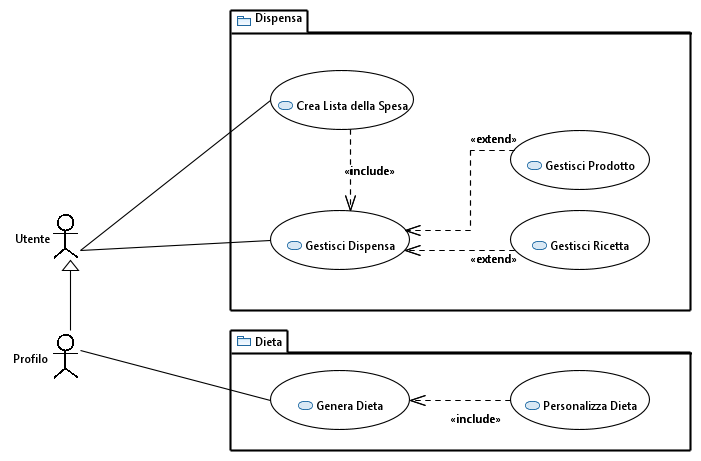
\includegraphics[width=\textwidth]{imgs/DiagrammaDeiCasiDUso_0.png}
    \caption{Diagramma dei casi d'uso}
    \label{fig:enter-label}
\end{figure}


%Si intende comunque mettere a disposizione in versioni future del software funzionalità più approfondite dal punto di vista tecnico, che si confida aggiungeranno valore per gli utenti più esperti e pratici.   

\subsection{Definizioni}
\textit{In ordine alfabetico}
\begin{center}
    \begin{tabular}{p{50pt}p{300pt}}
    \toprule
         \textbf{\textit{\hypertarget{caloria}{Chilocaloria [kcal]}}} & Rappresenta la quantità di calore necessaria per innalzare la temperatura di 1 Kg di acqua distillata da 14,5°C a 15,5°C. Viene utilizzata in ambito alimentare come metrica per il potere calorico contenuto negli alimenti, cioè per misurare quanta "energia" è contenuta nell'alimento. \\
         \textbf{\textit{\hypertarget{dispensa}Dispensa}} & Nominativo con cui ci si riferisce all'inventario attuale dell'utente (e quindi all'insieme dei prodotti alimentari, di qualsiasi genere, di cui l'utente vuole tenere traccia)    \\
         \textbf{\textit{\hypertarget{sweb}{Servizio Web\newline Esterno}}} & Si riferisce all'utilizzo di una connessione Internet per ricercare in rete un informazione mancante, attraverso l'invio di una richiesta (HTTP) ad un ente in grado di fornire il dato. \\ 
         \textbf{\textit{\hypertarget{unità}{Unità}}} & Si riferisce alla più piccola parte ("atomica") di un prodotto, al livello di dettaglio che interessa all'utente, cioè al singolo barattolo/bottiglia/confezione/sacchetto/busta/frutto/vegetale/cassetta\newline /scatola etc. \\ 
    \bottomrule
    \end{tabular} 
\end{center}
\subsection{Abbreviazioni}
\begin{center}
    \begin{tabular}{p{50pt}p{300pt}}
    \toprule
         \textit{FUNZ} & Requisiti funzionali  \\
         \textit{GUI} & Requisiti dell'interfaccia grafica  \\
    \bottomrule
    \end{tabular} 
\end{center}

\subsection{Priorità}
Nella tabella dei requisiti della sezione $2.6$ viene specificata, oltre all'ID del requisito ed alla sua descrizione, la priorità attribuita ad esso, secondo lo schema MoSCoW, per il quale si possono suddividere i requisiti in 
\begin{itemize}
    \item \textbf{Must Have} - requisiti assolutamente necessari. Verrà indicato con \hspace{.1cm} \begin{tabular}{c}
    \rowcolor{Green}
         M  \\ 
    \end{tabular}
    \item \textbf{Should Have} - requisiti importanti, ma non assolutamente necessari per un sistema utilizzabile. Verrà indicato con \hspace{.1cm} \begin{tabular}{c}
    \rowcolor{LimeGreen}
         S  \\ 
    \end{tabular}
    \item \textbf{Could Have} - requisiti che vengono implementati solo se il tempo lo consente. Verrà indicato con \hspace{.1cm} \begin{tabular}{c}
    \rowcolor{RedOrange}
         C  \\ 
    \end{tabular}
    \item \textbf{Won't Have} - requisiti non richiesti che rimarranno per la prossima iterazione. Verrà indicato con \hspace{.1cm} \begin{tabular}{c}
    \rowcolor{BrickRed}
         W  \\ 
    \end{tabular}
\end{itemize}


\subsection{Requisiti}
\paragraph{Funzionali}

\begin{center}
    \begin{longtable}{p{50pt}p{250pt}c}
    \toprule
        ID & Descrizione & Priorità \\
        \midrule
         \textit{FUNZ.1} & Il sistema dovrebbe utilizzare una \textit{\hyperlink{dispensa}{Dispensa}} per tenere traccia dei prodotti in possesso dell'utente. & \must  \\
         \textit{FUNZ.2} & Il sistema dovrebbe permettere di aggiungere/modificare/rimuovere un prodotto dalla \textit{Dispensa}. & \must \\
         \textit{FUNZ.3} & Il sistema dovrebbe tenere traccia, per ogni prodotto, delle seguenti informazioni:
         \begin{itemize}
             \item Data di acquisto/aggiunta
             \item Data di scadenza
             \item Quantità (peso, in chilogrammi/grammi [$kg$,$g$], volume, in litri/millilitri [$L$,$ml$] o numero di \textbf{\textit{\hyperlink{unità}{Unità}}})
             \item Calorie per quantità (in chilocalorie per $100g$ di prodotto [$\sfrac{\hyperlink{caloria}{kcal}}{100g}$])
         \end{itemize}& \must \\
         \textit{FUNZ.3.1} & Il peso viene memorizzato con una precisione fino alla terza cifra decimale e fino ad un tetto massimo di ??? $kg$, cioè da $0.001 = 1 g$ a $??? kg = ???g$ & \must\\
         \textit{FUNZ.3.2} & Il volume viene memorizzato con una precisione fino alla terza cifra decimale e fino ad un tetto massimo di ??? $L$, cioè da $0.001 L = 1 ml$ a $??? L = ???ml$.& \must \\
         \textit{FUNZ.3.3} & Le \textit{\hyperlink{unità}{Unità}} vengono memorizzate fino ad un numero massimo di ??? \textit{Unità}. &\must \\
         \textit{FUNZ.4} & Il sistema dovrebbe contenere già al suo interno le informazioni per prodotto riportate nel requisito \textit{FUNZ.3} degli alimenti più comuni.  & \should \\
         \textit{FUNZ.5} & Il sistema dovrebbe poter recuperare le informazioni per prodotto riportate nel requisito \textit{FUNZ.3} utilizzando un \textit{Servizio Web Esterno}, indipendente dall'applicazione. & \wont  \\
         \textit{FUNZ.6} & Il sistema dovrebbe permettere all'utente di aggiornare/modificare/cancellare le informazioni riportate nel requisito \textit{FUNZ.3} per ogni prodotto. & \must \\
         \textit{FUNZ.7} & Il sistema dovrebbe permettere di aggiungere/modificare/eliminare ricette. Per ogni ricetta il sistema memorizza i seguenti dati
         \begin{itemize}
             \item Quantità (per ingrediente)
             \item Note di preparazione
             \item Tempo di preparazione (in minuti [$min$])
         \end{itemize}& \should \\
         \textit{FUNZ.8} & Il sistema dovrebbe permettere di impostare l'obiettivo calorico giornaliero per l'utente principale.  & \must \\
         \textit{FUNZ.9} & Il sistema dovrebbe essere in grado di calcolare (in modo approssimativo) il fabbisogno calorico necessario per l'utente, utilizzando i seguenti parametri (inseriti dall'utente): \begin{itemize}
             \item Peso dell'individuo (in chilogrammi)
             \item Altezza dell'individuo (in centimetri)
             \item Attività fisica svolta 
             \begin{itemize}
                 \item Tipo di attività 
                 \item Durata dell'esercizio (minuti)
             \end{itemize}
         \end{itemize}  & \wont \\
         \textit{FUNZ.10} & Il sistema dovrebbe permettere di impostare il numero di individui di cui vuole tenere traccia. & \could \\
         \textit{FUNZ.10.1} & Il sistema dovrebbe permettere di impostare l'obiettivo calorico giornaliero per ogni individuo.  & \could \\
         \textit{FUNZ.11} & Il sistema dovrebbe permettere di creare una \textit{Lista della spesa} in cui l'utente può aggiungere prodotti che ha intenzione/necessità di acquistare. & \could \\
         \textit{FUNZ.12} & Il sistema dovrebbe permette di recuperare ricette attraverso un Servizio Web esterno, e proporle all'utente. & \wont \\
         \textit{FUNZ.13} & Il sistema dovrebbe notificare l'utente quando un prodotto sta per scadere. & \must \\
         \textit{FUNZ.13.1} & La notifica verrà inviata ??? giorni prima della scadenza. & \should  \\
         \textit{FUNZ.14} & Il sistema dovrebbe permettere all'utente di rimuovere velocemente i prodotti che ha utilizzato. & \should \\
         \bottomrule
    \end{longtable} 
\end{center}

\paragraph{Graphic User Interface (GUI)}
\begin{center}
    \begin{tabular}{p{50pt}p{250pt}c}
    \toprule
        ID & Descrizione & Priorità \\
        \midrule
         \textit{GUI.1} & L'interfaccia utente dovrebbe rispondere in modo reattivo agli input dell'utente, fornendo un feedback visivo. & \should \\
         \textit{GUI.2} & La data di scadenza dei prodotti sarà segnata \begin{itemize}
             \item In giallo per i prodotti in scadenza (cioè a ??? giorni dalla data limite)
             \item In rosso per i prodotti che hanno superato la data di scadenza
         \end{itemize} & \should \\
         \textit{GUI.3} & Il requisito \textit{FUNZ.14} dovrebbe essere soddisfatto ponendo un pulsante "+" e un pulsante "-" sotto le immagini dei prodotti. & \could \\
         \textit{GUI.4} & L'interfaccia dovrebbe disporre di una schermata principale detta "Schermata Home" & \must  \\
         \textit{GUI.4.1} & La Schermata Home dovrebbe mostrare i prodotti e disporli in un ordinamento a matrice o ad elenco. & \must \\
         \textit{GUI.5} & In caso l'applicazione vada in background, o venga sospesa, quando viene riattivata deve tornare all'ultima schermata su cui era prima della sospensione. & \wont \\
         \bottomrule
    \end{tabular} 
\end{center}

\section{UML}
Si rappresentano di seguito i diagrammi UML delle Macchine a Stati Finiti che modellano alcune parti del software; in particolare vengono rappresentati gli stati in cui dovrebbe trovarsi l'interfaccia grafica per l'utente (GUI, \textit{Figure 2}), e i possibili stati di un prodotto della dispensa (\textit{Figure 3}). 

\begin{figure}[H]
    \centering
    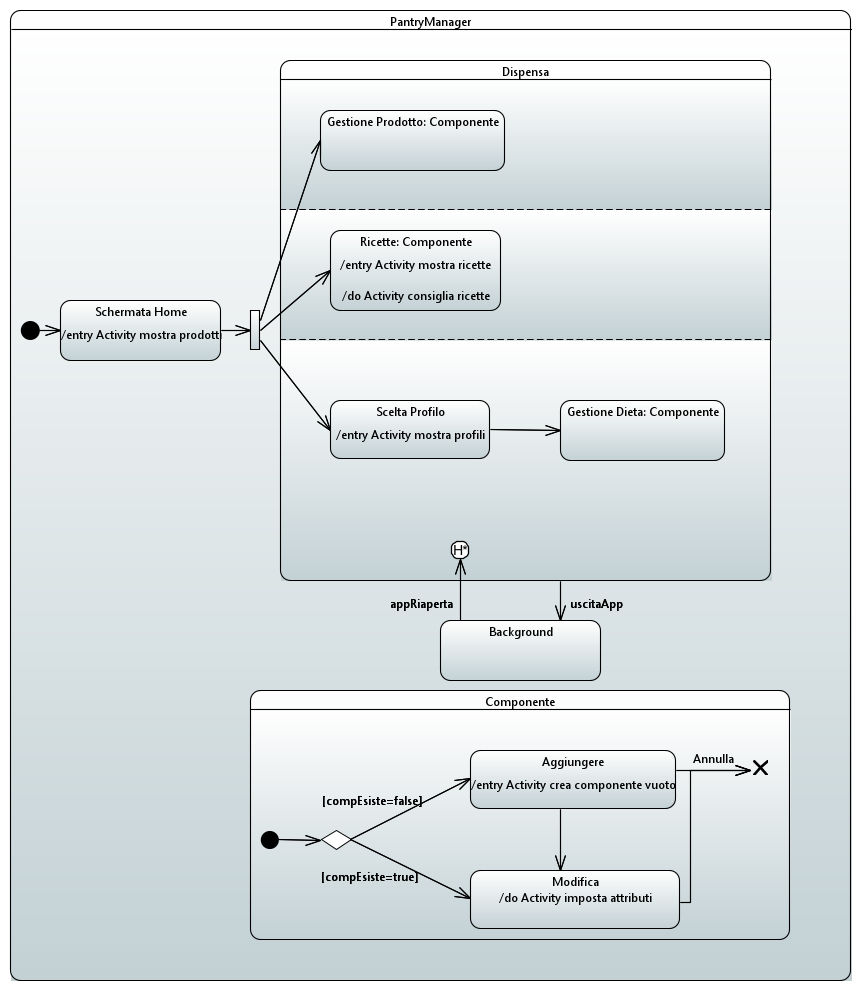
\includegraphics[width=\linewidth]{imgs/GUISttMchnDgrm.png}
    \caption{GUI State Machine Diagram}
    \label{fig:enter-label}
\end{figure}
\begin{figure}[H]
    \centering
    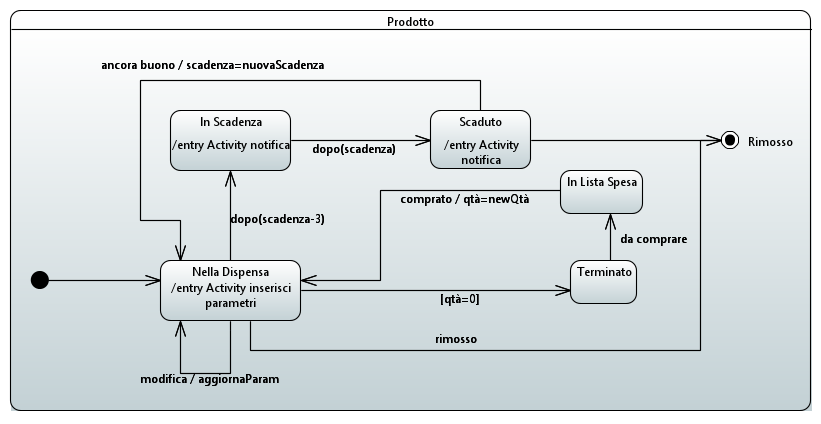
\includegraphics[width=\linewidth]{imgs/ProdottoSttMchnDgrm.png}
    \caption{Product State Machine Diagram}
    \label{fig:enter-label}
\end{figure}

\textit{\textcolor{black!60}{La visione dei modelli UML è disponibile anche dal repository Github del progetto.}}

\section{Qualità del Software}
Si è deciso di non adottare uno standard predefinito per la definizione dei requisiti di qualità, poiché si ritiene che l'effettiva verifica tecnica del soddisfacimento della qualità richiesta non risulti fattibile; si è comunque deciso di definire dei "principi" generici che mostrino gli obiettivi che hanno guidato lo sviluppo.

\begin{itemize}
    \item Si intende sviluppare un'interfaccia reattiva, per questo si punta verso un design dell'interfaccia grafica semplice e meno appetibile, ma comunque veloce. 
    \item Si intende sviluppare un sistema che garantisca un livello di sicurezza almeno sufficiente, cioè non richieda privilegi avanzati di accesso alla memoria del dispositivo su cui è installato, e, inoltre, non acceda a dati sensibili dell'utente (se non quelli da quest'ultimo dichiarati)
    \item Il sistema non dovrebbe mostrare malfunzionamenti o prestazioni pessime, nella maggior parte dei casi: si punta ad una presenza minima di \textit{lag} nell'interfaccia, \textit{crash} inaspettati e rallentamenti non trascurabili. 
\end{itemize}

\end{document}
